\documentclass{math}

\usepackage{tikz}

\title{University Physics 1A}
\author{Alvin Lin}
\date{November 27th, 2017}

\begin{document}

\maketitle

\section*{Test Review}
A ball of mass \( m \) is thrown vertically upwards with an initial speed
\( v_0 \) a horizontal distance \( d \) from a point \( O \) on the level
ground. As it moves upwards, find an expression for the angular momentum of
the ball as a function of the height relative to point \( O \).
\begin{align*}
  L &= \vec{r}\times m\vec{v} \\
  &= \langle d,h\rangle\times m\langle0,v\rangle \\
  &= \begin{vmatrix}
    \i & \j & \k \\
    d & h & 0 \\
    0 & mv & 0
  \end{vmatrix} \\
  &= \langle0,0,dmv\rangle \\
  v(h) &= \sqrt{v_0^2-2ah} \\
  L(h) &= \left\langle0,0,dm\sqrt{v_0^2-2gh}\right\rangle
\end{align*}

\subsection*{Review Problem}
A solid disk is mounted so it can rotate without friction about an axis through
its center. Initially it rotates with some angular velocity \( \omega \). A
second circular object, initially not rotating, is dropped concentrically onto
the disk. The second object has the same mass and radius as the disk. When the
two come to a common rotation, the final angular velocity is \( \frac{1}{3} \)
of the original. What is the shape of the second object?
\begin{align*}
  I_1\omega &= (I_1+I_2)\frac{1}{3}\omega \\
  3I_1 &= I_1+I_2 \\
  2I_1 &= I_2 \\
  2(\frac{1}{2}MR^2) &= MR^2
\end{align*}
The second object is a thin walled cylinder.

\subsection*{Review Problem}
A thin rod of mass 9.0kg and length 0.80m is pivoted at one end and can
rotate without friction along a horizontal surface. The diagram is a top view.
Initially it is rotating clockwise at \( 1.2\frac{rad}{s} \). A piece of putty
of mass 50g slides without friction toward the end of the rod as shown with
a speed of \( 60\frac{m}{s} \). The putty collides and sticks to the rod at
the very end. What is the final angular velocity of the rod and putty?
\begin{center}
  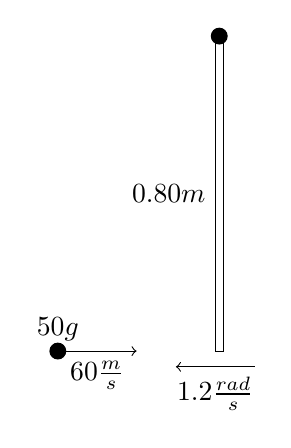
\begin{tikzpicture}
    \draw[fill=black] (0.05,0) circle (0.1cm);
    \draw (0,0) -- (0.1,0) -- (0.1,-4) -- (0,-4) -- cycle node[pos=0.5,left]
      {\( 0.80m \)};
    \draw[->] (0.5,-4.2) -- (-0.5,-4.2) node[pos=0.5,below]
      {\( 1.2\frac{rad}{s} \)};
    \draw[fill=black] (-2,-4) circle (0.1cm) node[above] {\( 50g \)};
    \draw[->] (-2,-4) -- (-1,-4) node[pos=0.5,below] {\( 60\frac{m}{s} \)};
  \end{tikzpicture}
\end{center}
\begin{align*}
  L_{putty}-L_{rod} &= L_{rod+putty} \\
  dmv-I\omega &= I_{rod+putty}\omega_{final} \\
  (0.8)(0.05)(60)-\frac{1}{3}(9)(0.8^2)(1.2) &=
    (\frac{1}{3}(9)(0.8)^2+(0.05)(0.8)^2)\omega_{final} \\
  \omega_{final} &= \frac{2.4-2.304}{1.952} \\
  &= 0.049\frac{rad}{s}
\end{align*}
The same rod is hung vertically, and now it is initially at rest. The same
piece of putty is show at the bottom end with some speed, hits the rod and
sticks to it, and now the rod plus putty swings up. When the rod and putty
momentarily come to rest, the rod makes an angle of \( 76^{\circ} \) with the
vertical. What is the speed of the putty?
\begin{align*}
  mvL &= \left(\frac{1}{3}ML^2+mL\right)\omega_{rod+putty} \\
  \frac{1}{2}I\omega^2 &=
    \frac{1}{2}\left(\frac{1}{3}ML^2+mL^2\right)\omega^2 \\
  &= 0+mg\bigg[L(1-\cos\theta)\bigg]+
    Mg\left[\frac{1}{2}L(1-\cos\theta)\right] \\
\end{align*}
Plug in the first equation (angular momentum) into the second equation
(conservation of energy) to solve for the speed of the putty.

\begin{center}
  You can find all my notes at \url{http://omgimanerd.tech/notes}. If you have
  any questions, comments, or concerns, please contact me at
  alvin@omgimanerd.tech
\end{center}

\end{document}
